\documentclass{article}
\usepackage[utf8]{inputenc}

\title{IF683 - Projeto de Desenvolvimento}
\author{Henrique de Oliveira Braga Sakane }
\date{Outubro 2018}

\usepackage{natbib}
\usepackage{graphicx}

\begin{document}

\maketitle

\section{Introdução}
A disciplina Projeto de Desenvolvimento tem como foco principal o desenvolvimento de projetos de computação a partir de conceitos estudados em semestres anteriores dos cursos de Ciência da Computação e Engenharia da Computação da UFPE.

Essa disciplina é oferecida para alunos do 5º período de C.C. e 8º período de E.C. , além do curso de Design da UFPE. Ela é dada pelos professores André Neves, Cristiano Coêlho de Araújo e Geber Ramalho.

\section{Relevância}
A disciplina Projeto de Desenvolvimento é cadeira obrigatória pois é de grande importância quando se trata da área de criatividade no desenvolvimento de projetos.

A cadeira estimula o lado empreendedor do aluno, abrindo novos caminhos para a criação de empresas juniores e Startups, além incentivar os estudantes a trabalharem em equipe.O calendário da disciplina é preenchido de seminários essenciais para o desenvolvimento das pesquisas.


\section{Cadeiras Relacionadas}
\begin{table}[h]
    \centering
    \begin{tabular}{l|c|}
    Disciplina & Relação \\
    \hline
    IF669 - Introdução a Programação & Estudar programação para desenvolver\\  &  projetos. \\
    \hline
    IF676 - Metodol Expressão Tec-Cientifica & Está diretamente relacionada \\  & a areá de pesquisa e métodos científicos. 
    \end{tabular}
    \label{tab:my_label}
\end{table}

\begin{figure}[h!]
\centering
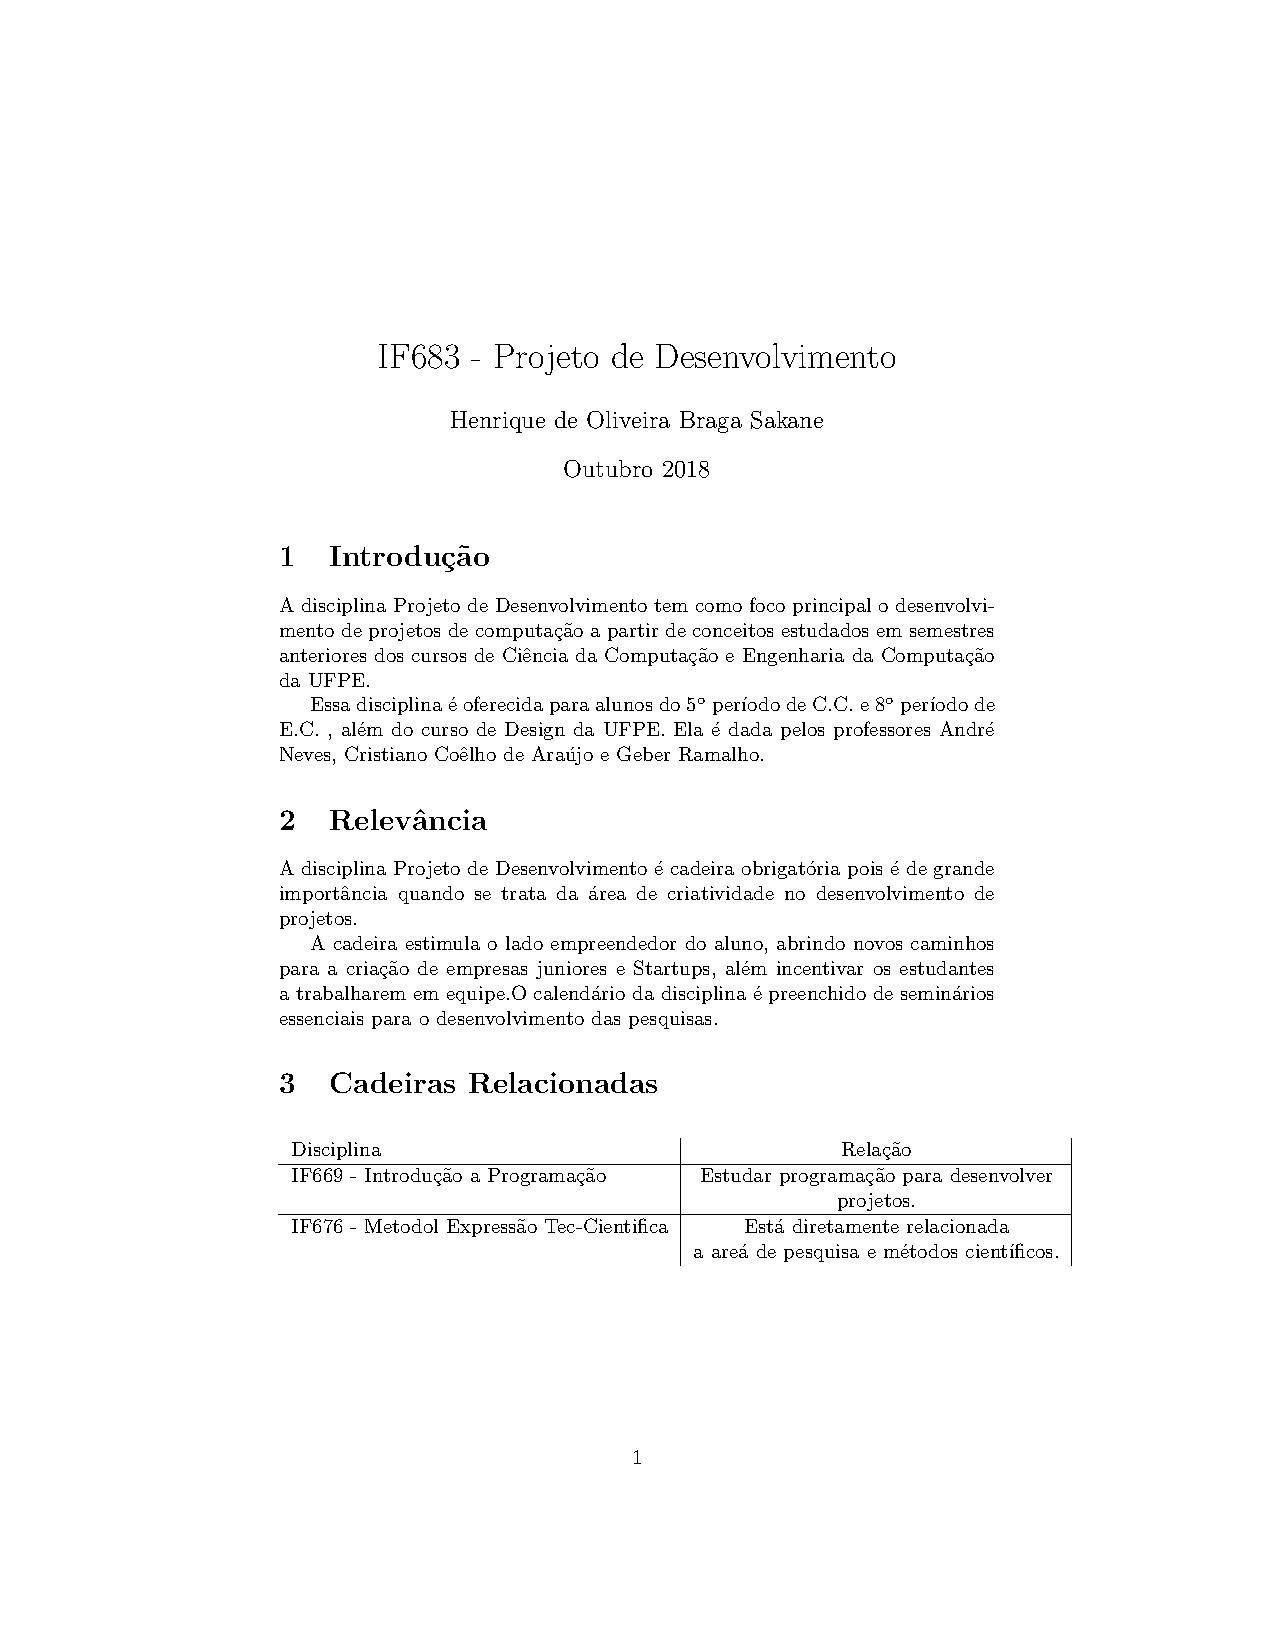
\includegraphics[scale=1.0]{hobs}
\caption{Planejamento e Pesquisa | Licença: Domínio Público}
\label{fig:hobs}
\end{figure}

\bibliographystyle{alpha}
\bibliography{hobs}
\cite{BlueOceanStrategy}
\cite{BusinessModelGeneration}
\cite{InnovationandEntrepreneurship}
\cite{TheLeanStartup}
\end{document}
